\section{Kinetyka fizyczna}
\subsection{Równania transportowe Własowa [Vlasova] i Boltzmana}
Funkcja rozkładu $\f$ na przestrzeni $\mu,\ \dim[\mu]=6.$
\begin{equation} \f d^3rd^3p = \f d^6\omega \implies d^6\omega 
= d^3rd^3p \end{equation}
\begin{equation} \int d^3rd^p\f = N(t) \end{equation}
Dalej dla uproszczenia piszemy samo $N$ pamiętając o zależności czasowej.\\

\textbf{Dla gazu \underline{jednorodnego}:}
$$ \int d^3rd^3p \f = \int d^3rd^3pf(\vec{p},t) = V \int d^3p f(\vec{p},t)=N.$$
\begin{equation}
\int d^3p f(\vec{p},t) = \frac{N}{V} = n \mbox{ - koncentracja cząstek.}
\end{equation}
Oraz
\begin{equation}
N = \frac{\mbox{objętość układu}}{\mbox{objętość na jedną cząstkę}} \equiv 
\frac{V}{v}.
\end{equation}
Dla małego układu 
\begin{equation}
v=\frac{4}{3} \pi r_s^3 ,
\end{equation}
gdzie $r_s$ to promień kulki w jakiej możemy zamknąć jedną cząstkę. Stąd
$$ n = \frac{V}{v} \implies v=\frac{V}{N} = \frac{1}{n}$$
$$ \frac{4}{3} \pi r_s^3 = \frac{1}{n} \implies r_s = \left[ \frac{3}{4\pi n}
\right]^{1/3} \propto n^{-1/3}.$$
\begin{center}
\begin{minipage}{0.3\textwidth}
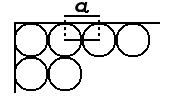
\includegraphics[width=5cm]{kuleczki_z_atomami.png}
\end{minipage}
\begin{minipage}{0.4\textwidth}
średnia odległość $a=2r_s$ \\
między cząsteczkami w gazie \\
o koncentracji $n$ \\
$$a \propto n^{-1/3}$$ \vspace{-5mm}\\
\end{minipage}
\end{center}

\textbf{Dla gazu \underline{niejednorodnego}:}
\begin{equation}
\int d^3rd^3\f = \int d^3r n(\vec{r}) = N \implies n(\vec{r}) 
\mbox{ - gęstość cząstek w } \vec{r}.
\end{equation}
\subsection{Zespoły statysyczne i przestrzeń fazowa $\Gamma$}

